\section{I/O-Streams}
\verb|java.io.*|\\
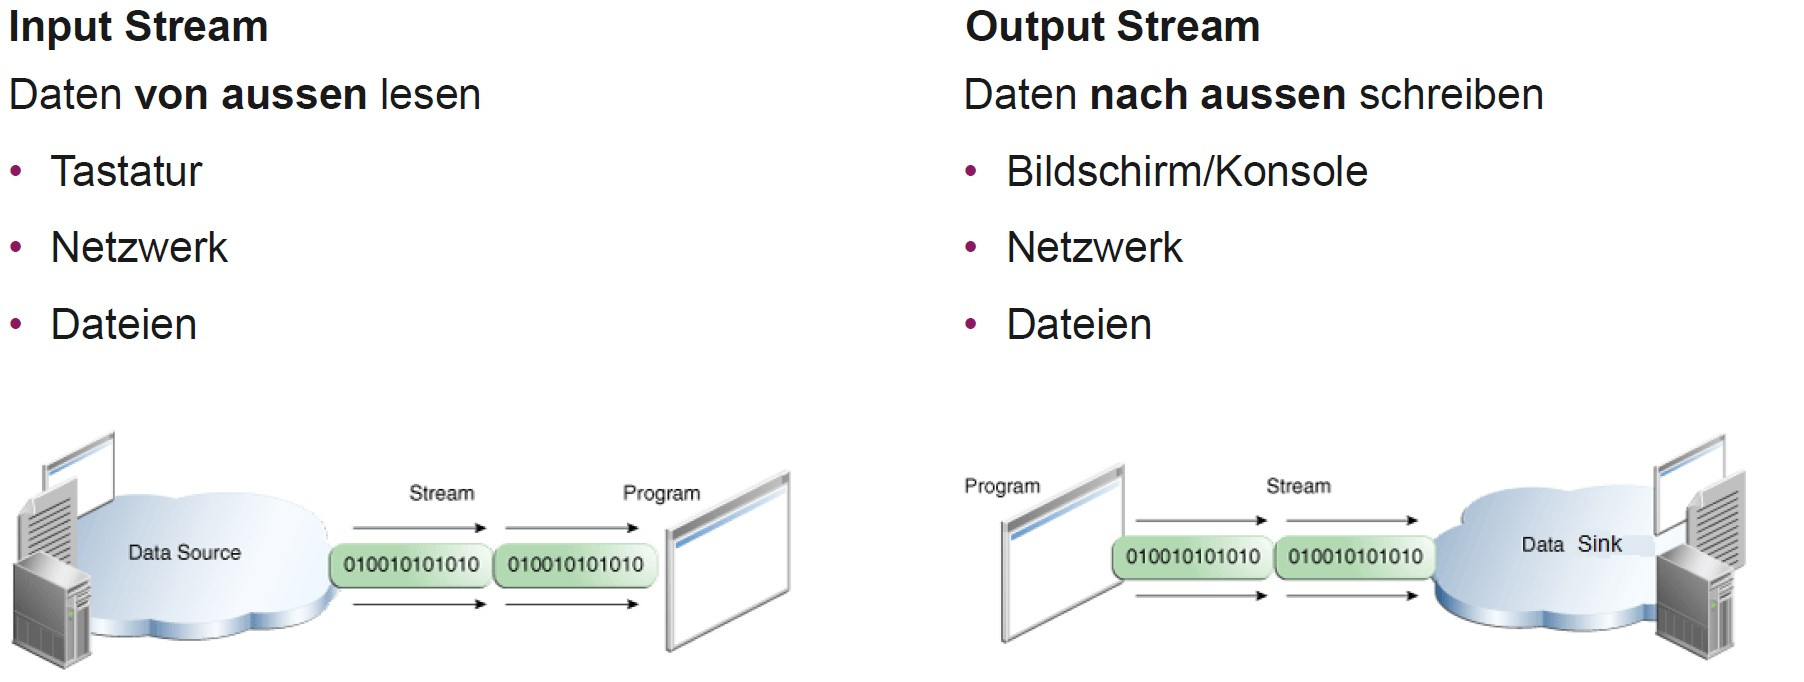
\includegraphics[width=0.9\linewidth]{pictures/streams.jpg}

Byte-Streams:
\begin{itemize}
    \itemsep0em
    \item 8-Bit-Daten
    \item Klassen erben von \verb|InputStream, OutputStream|
\end{itemize}

Character-Streams:
\begin{itemize}
    \itemsep0em
    \item 16-Bit Textzeichen (UTF-16)
    \item Klassen erben von \verb|Reader, Writer|
    \item Zeichen- / Zeilenweise Ein- \& Ausgabe
\end{itemize}

\subsection{Byte-Streams}
\textbf{InputStream}: \verb|int read(byte[] b, int offset, int length)| \\
\textbf{OutputStream}: \verb|void write(byte[] b, int offset, int length)| \\
Lese/schreibe \verb|length| Bytes in Array \verb|b| ab Index \verb|offset|\\
\\
\verb|void flush()|: Implizit bei \verb|close()|

\subsubsection{Standard Input/Output}
\verb|System.in| von \textit{InputStream}

\verb|System.out| und \verb|System.err| von \textit{PrintStream} (Subklasse von \textit{OutputStream})

\subsubsection{FileInput}
Ganze Datei binär einlesen (kann speicherintensiv werden):\\
\verb|byte[] data = Files.readAllBytes(Path.of("in.bin"));|
\hrule
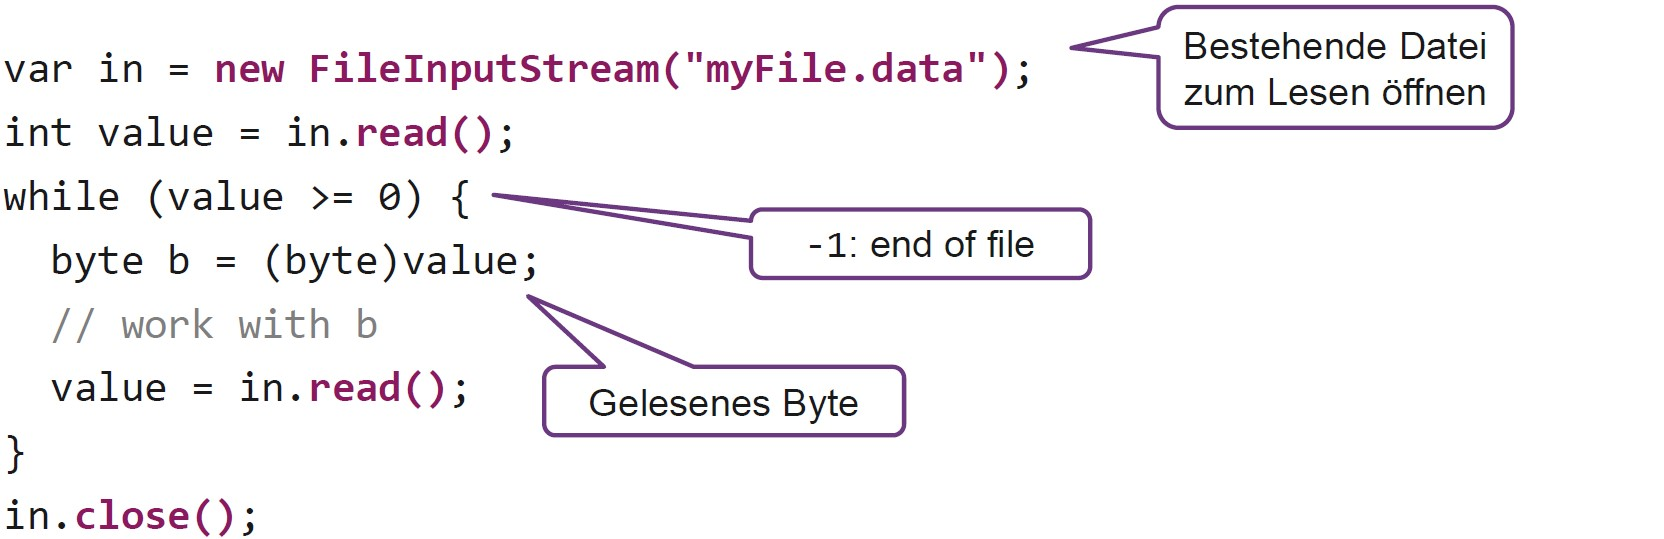
\includegraphics[width=0.9\linewidth]{pictures/file-in.jpg}


\subsubsection{FileOutput}
Ganze Datei binär schreiben:\\
\verb|Files.write(Path.of("out.bin"), data);|
\hrule
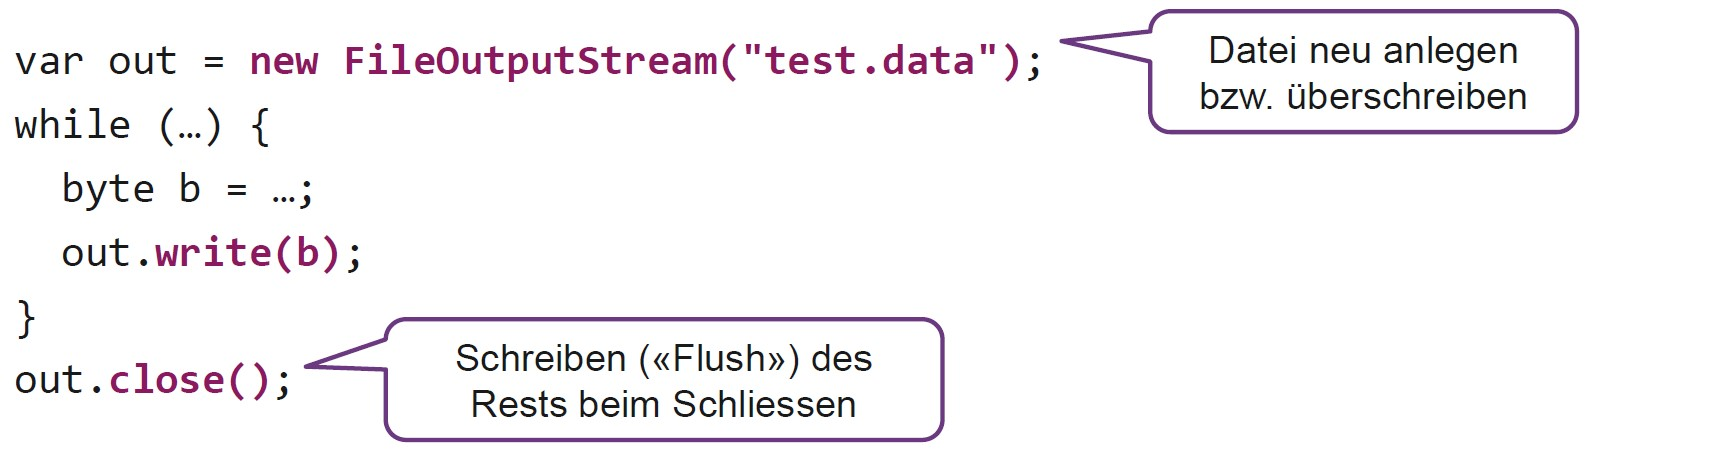
\includegraphics[width=0.9\linewidth]{pictures/file-out.jpg}

\verb|new FileOutputStream("test.data", true)| um an existierende Datei anzuhängen

\subsection{Character-Stream}

\subsubsection{FileReader}
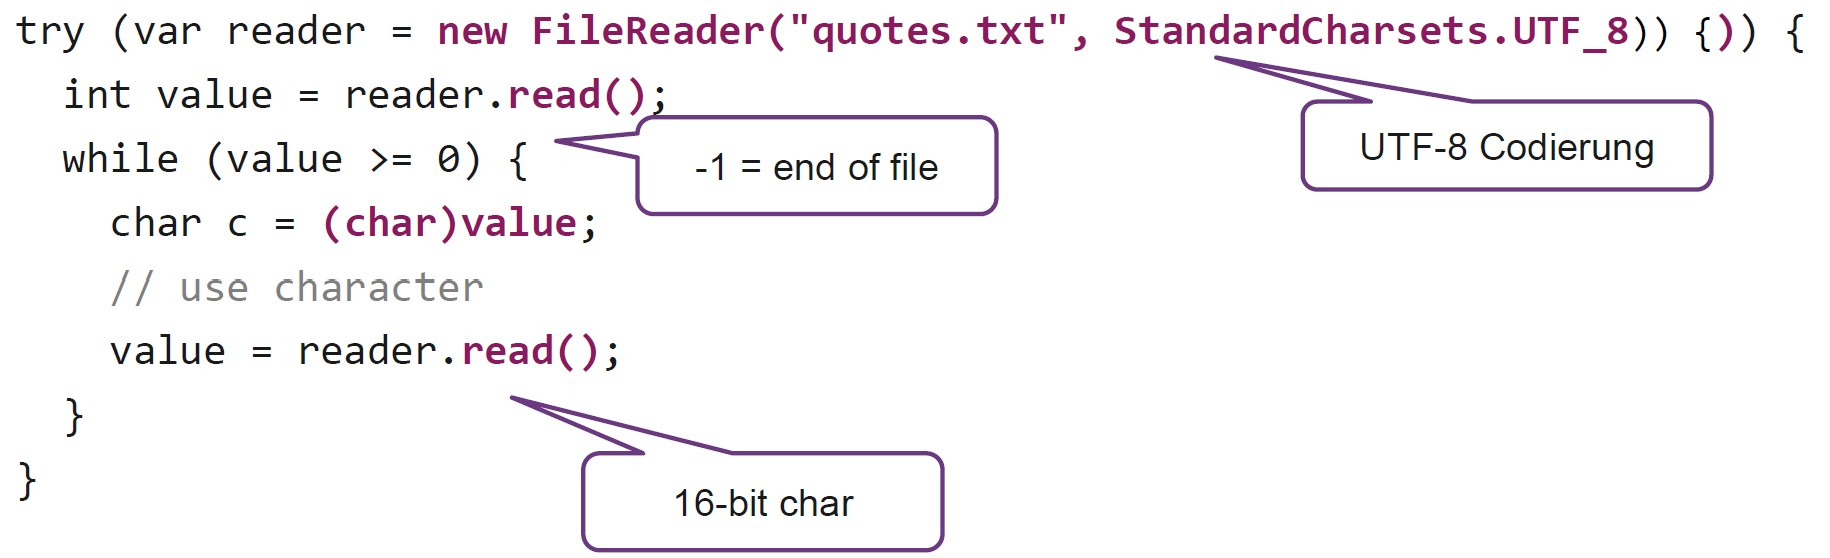
\includegraphics[width=0.9\linewidth]{pictures/filereader.jpg}\\
\verb|new FileReader(f)| \\
$\updownarrow$ \\
\verb|new InputStreamReader(new FileInputStream(f))|

\subsubsection{FileWriter}
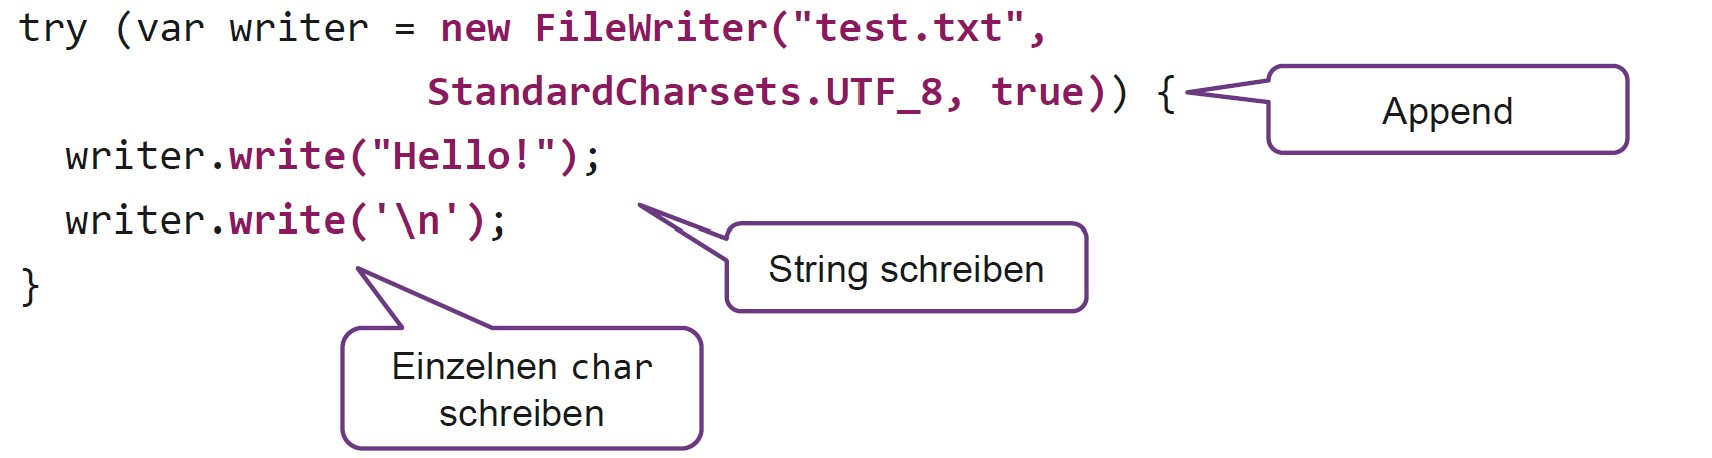
\includegraphics[width=0.9\linewidth]{pictures/filewriter.jpg}

\subsubsection{Zeilenweises Lesen}
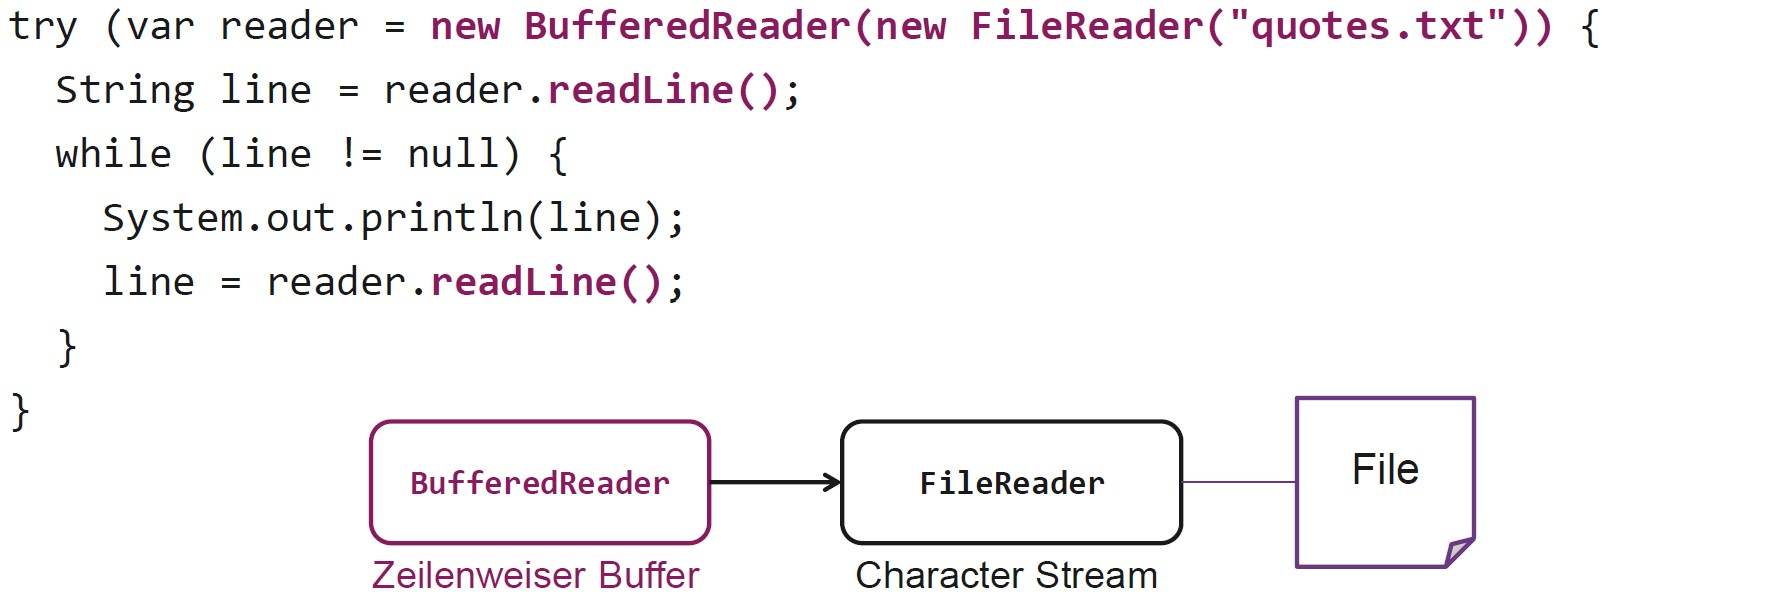
\includegraphics[width=0.9\linewidth]{pictures/zeilenweise.jpg}

\subsubsection{Einfachster Text-Datei-Zugriff}
\begin{tabular}{l}
    Ganze Text-Datei lesen \\
    \verb|List<String> lines = Files|\verb|.readAllLines(Path.of("in.txt"),| \\
    \verb|StandardCharsets.UTF_8);| \\
    \\
    Ganze Text-Datei schreiben \\
    \verb|Files.write(Path.of("out.txt"),| \\
    \verb|lines, StandardCharsets.UTF_8);| \\
\end{tabular}